\section{Theorie}
\label{sec:Theorie}

\subsection{Halbwertszeit}
\label{ssec:t1}

Atomkerne können unter Umständen sehr instabil werden.
Variieren die Verhältnisse von Protonen und Neutronen zu sehr, kann es passieren, dass der Kern zerfällt.
Dabei kann er entweder in einen stabilen Zustand zerfallen, oder in einen Zwischenzustand, der ebenfalls durch einen Zerfall in einen neuen Zustand übergeht.
Es ist unmöglich zu sagen, wann genau dies bei einem einzelen Atom passiert.
Allerdings ist es möglich bei einer großen Anzahl an Kernen eine Aussage über die Anzahl der nicht zerfallenden Kerne zu treffen.
Nachdem die sogenannte Halbwertszeit $T$ verstrichen ist, sind noch die Hälfte der Kerne nicht zerfallen.
Diese Größe kann je nach Kern über 23 Größenordnungen variieren.
Um diesen Prozess und somit auch die Messung der Halbwertszeit zu verstehen, wird im Folgenden erklärt wie die instabilen Kerne genau funktionieren.

\subsection{Kernreaktionen mit Neutronen}
\label{ssec:t2}

Die instabilen Kerne müssen zunächst erzeugt werden.
Einige von ihnen zerfallen so schnell, dass sie optimalerweise kurz vor der Messung erzeugt werden.
Dafür werden Neutronen auf stabile Kerne geschossen.
Der Kern nimmt die kinetische Energie auf und verteilt sie auf seine Nukleonen. 
Es ist jetzt nicht möglich ein Nukleon abzustoßen, also gibt der Kern ein Photon $\gamma$ ab.
Damit begibt er sich in seinen Grundzustand zurück. 

$\ce{^{m}_zA + ^{1}_0n -> ^{m+1}_zA + \symup{\gamma}}$

Wegen des neuen Neutrons ist auch dieser Kern nicht dauerhaft stabil und zerfällt schließlich auch, dabei emittiert er ein Elektron und ein Antineutrino. 
Beide Teilchen teilen sich die Energie, die nach diesem Prozess überschüssig wäre.

$  \ce{  ^{m+1}_zA -> ^{m+1}_{z+1}C + \symup{\beta}- + E_{Kin} + \bar{\symup{\nu}}_e}   $

Ein weiterer wichtiger Begriff ist der Wirkungsquerschnitt $\sigma$. 
Dieser gibt eine Fläche an, in der jedes auf diese Fläche treffende Neutron eingefangen wird.
Wird eine dünne Folie mit einer Fläche von $\SI{1}{\square\centi\metre}$ mit der Dicke $d$ und einer Anzahl Atome K pro $\si{\cubic\centi\metre}$ von $n$ Neutronen pro Sekunde getroffen, ergibt sich der Wirkungsquerschnitt 


\begin{equation}
    \sigma = \frac{u}{n \; K\; d}.
    \label{eq:sigma}
\end{equation}

Wobei $u$ die Anzahl der Kerne ist, die tatsächlich einschlagen.
%Die Geschwindigkeit $v$ der Neutronen beeinfluss den Wirkungsquerschnitt ebenfalls, daher muss dort zwischen %schnellen und langsamen Teilchen unterschieden werden.
%Über die De-Broglie Wellenlänge $\lambda$ kann entschieden werden, wie weiter vorgegangen wird.
%Wenn $m_\text{n}$ die Neutronenmasse ist und $h$ das Plancksche Wirkungsquantum, ist die De-Broglie Wellenlänge über 
%
%\begin{equation}
%    \lambda = \frac{h}{m_\text{n} \cdot v}.
%    \label{eq:debroglie}
%\end{equation}
%
%gegeben.
%Ist sie klein gegen den Kernradius kann die Reaktion des Neutron auf den Kern mit simplen geometrischen Rechnungen %gelöst werden, ist sie hingegen groß gegen den Radius müssen Interferenzeffekte beachet werden.
%Der Wirkungsquerschnitt wird dann in Abhängigkeit von der Neutronenergie $E$ berechnet.



\subsection{Erzeugung niederenergetischer Neutronen}
\label{ssec:t3}

Um niederenergetische Neutronen zu erzeugen werden andere Kernreaktionen dafür genutzt.
In diesem Versuch wird die Reaktion 

$\ce{^{9}_{4}Be + ^{4}_{2}\symup{\alpha} -> ^{12}_{6}C + ^{1}_0n}$

verwendet.
Nach dieser Reaktion sind die Neutronen allerdings hochenergetisch, also werden sie gebremst.
Es wird eine Aperatur wie in \autoref{fig:therm} verwendet.
Dort werden die entstandenen Neutronen durch Parafin geschickt, es besteht größtenteils aus Wasserstoff, dem idealen Stoßpartner für die Neutronen.

\begin{figure}
    \centering
    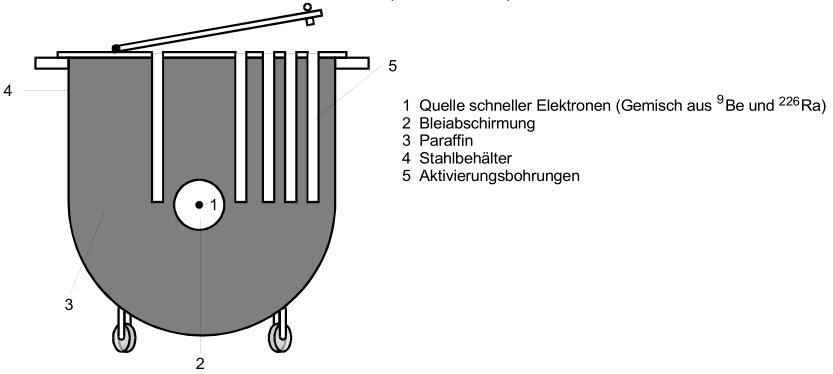
\includegraphics[width=\textwidth]{images/bild1.png}
    \caption{Querschnitt einer Quelle für thermische Neutronen.\cite{V702}}
    \label{fig:therm}
\end{figure}

Bei einer Temperatur von $\SI{290}{\kelvin}$ besitzen sie dann noch eine Energie von etwa $\SI{0.025}{\electronvolt}$.
Neutronen mit so einer Energie werden thermische Elektronen genannt.

\subsection{Untersuchung des Zerfalls instabiler Isotope}
\label{ssec:t4}

Die eigentliche Analyse der Isotope kann nun beginnen, im folgenden werden Vanadium und Rhodium Isotope betrachtet.
Diese werden in die Aktivierungsschächte in \autoref{fig:therm} gesteckt.
Dort werden sie dann durch Neutronenbeschuss instabil und es wird der daraufhin auftretende Zerfall gemessen.
Der Zerfall von Vanadium ist

$\ce{^{51}_{23}V + ^{1}_0n -> ^{52}_{23}V -> ^{52}_{24}Cr + \symup{\beta}- + \bar{\symup{\nu}}_e}$.

Wegen des Neutronenüberschusses wandelt sich eines von ihnen in ein Proton, Elektron und ein Elektronen-Antineutrino um.

$\ce{^{1}_0n -> ^{1}_1p + e- \bar{\symup{\nu}}_e}$

Dadurch entsteht das stabile Chrom.
Dieser Zerfall wird über die Funktion 

\begin{equation}
    N \left(t\right) = N_0 \cdot \exp(-\lambda T)
    \label{eq:zerfall}
\end{equation}

untersucht.
$N$ gibt die Anzahl der noch nicht zerfallenen Kerne an und $N_0$ die Anzahl der bei $t = 0$ vorliegenden Kerne.
$\lambda$ ist hier die Zerfallskonstante.
Sie ist über die Halbwertszeit 

\begin{equation}
    T = \frac{\ln{2}}{\lambda}
    \label{eq:lambda}
\end{equation}

bestimmbar.
% Experimentell lässt sich $\lambda$ auch über eine Ausgleichsgerade der Form

% \begin{equation}
%     \ln{N_{\Delta \text{t}}\left(t\right)} = \ln{ N_0 \left(1 - \exp(-\lambda \Delta T) \right)} -\lambda T
%     \label{eq:lambda2}
% \end{equation}

% bestimmten, wenn eine Ausgleichsgerade durch die Messwerte gelegt wird.

Rhodium zerfällt nicht nur auf eine Art, daher müssen hier zwei Fälle unterschieden werden.
Zu $90\%$ zerfällt es wie

$\ce{^{103}_{45}Rh + ^{1}_0n -> ^{104}_{45}Rh -> ^{104}_{46}Pd + \symup{\beta}- + \bar{\symup{\nu}}_e}$

Dies ist der erwünschte Zerfall, der auch gemessen werden soll.
Es kann allerdings auch passieren, dass die Reaktion nach

$\ce{^{103}_{45}Rh + ^{1}_0n -> ^{104i}_{45}Rh -> ^{104}_{45}Rh + \symup{\gamma} -> ^{104}_{46}Pd + \symup{\beta}- + \bar{\symup{\nu}}_e}$

verläuft.
Dabei wird ein sogenannter isomerer Kern $\ce{^{104i}_{45}Rh}$ gebildet, der ein Photon aussendet und dadurch in einen anderen Zustand übergeht. 
Dieser Vorgang beeinflusst die Messung des ersten Zerfalls, trägt man die Messung beider Zerfälle auf, sieht es in etwa so aus, wie in \autoref{fig:zerfall}.

\begin{figure}
    \centering
    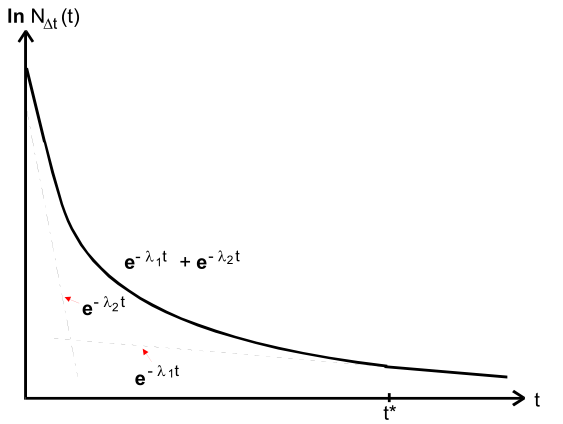
\includegraphics[width=0.6\textwidth]{images/bild2.png}
    \caption{Zerfallskurve mit zwei verschieden schnell ablaufenden Zerfällen.\cite{V702}}
    \label{fig:zerfall}
\end{figure}

Hier sind gleich zwei Zerfälle überlagert, ein kurzlebiger und ein langlebiger.
Für die Auswertung wird zunächst die Zerfallskonstante des langlebigens Zerfalls bestimmt.
Dann wird diese vom kurzlebigen Zerfall abgezogen.